\documentclass[11pt]{article}
\usepackage[utf8]{inputenc}
\usepackage[T1]{fontenc}
\usepackage{amsmath}
\usepackage{amssymb}
\usepackage{multicol}
\usepackage{geometry}
\usepackage{tikz}
\usepackage{enumitem}
\usepackage{xcolor}
\usepackage{titlesec}

% Configurações de layout
\geometry{a4paper, left=1cm, right=1cm, top=0.5cm, bottom=1.2cm}
\setlength{\columnseprule}{0.4pt}

% Cores para títulos
\titleformat{\section}{\normalfont\Large\bfseries\color{blue}}{\thesection}{1em}{}
\titleformat{\subsection}{\normalfont\large\bfseries\color{red}}{\thesubsection}{1em}{}

% Comandos personalizados
\newcommand{\respostaNum}[1]{\textcolor{blue}{\boxed{#1}}}
\newcommand{\respostaTxt}[1]{\textcolor{blue}{#1}}
\newcommand{\resolucao}{\textbf{\textcolor{blue}{Resolução:}}}

\title{\textcolor{red}{Gabarito Comentado: Medidas de Tendência Central}}
\author{Professor: Jefferson}
\date{}

\begin{document}

\maketitle
\vspace{-1cm}

\begin{multicols}{2}

\section*{Instruções}
\textbf{Verifique suas respostas e estude as resoluções comentadas.}

\section*{Gabarito - Exercícios Básicos}

\begin{enumerate}[leftmargin=*]

\item \textbf{Calcule a média aritmética dos seguintes conjuntos:}

\begin{enumerate}[label=\alph*)]
\item $4, 7, 9, 12, 18$

\resolucao
\[
\bar{x} = \frac{4 + 7 + 9 + 12 + 18}{5} = \frac{50}{5} = \respostaNum{10}
\]

\item $8, 8, 10, 12, 14, 18$

\resolucao
\[
\bar{x} = \frac{8 + 8 + 10 + 12 + 14 + 18}{6} = \frac{70}{6} \approx \respostaNum{11,67}
\]

\item $5, 10, 15, 20, 25$

\resolucao
\[
\bar{x} = \frac{5 + 10 + 15 + 20 + 25}{5} = \frac{75}{5} = \respostaNum{15}
\]
\end{enumerate}

\item \textbf{Determine a mediana dos conjuntos:}

\begin{enumerate}[label=\alph*)]
\item $6, 2, 8, 4, 10$ (ordene primeiro)

\resolucao Ordenando: $2, 4, 6, 8, 10$ ($n = 5$, ímpar)
\[
Md = \text{3º termo} = \respostaNum{6}
\]

\item $15, 20, 25, 30, 35, 40$

\resolucao Dados já ordenados ($n = 6$, par)
\[
Md = \frac{25 + 30}{2} = \frac{55}{2} = \respostaNum{27,5}
\]

\item $3, 7, 1, 9, 5, 8, 2$

\resolucao Ordenando: $1, 2, 3, 5, 7, 8, 9$ ($n = 7$, ímpar)
\[
Md = \text{4º termo} = \respostaNum{5}
\]
\end{enumerate}

\item \textbf{Encontre a moda dos conjuntos:}

\begin{enumerate}[label=\alph*)]
\item $4, 6, 4, 8, 4, 10, 6$

\resolucao Frequências: 4 aparece 3 vezes, 6 aparece 2 vezes, os demais 1 vez
\[
Mo = \respostaNum{4} \quad \text{(unimodal)}
\]

\item $12, 15, 18, 15, 20, 12, 25$

\resolucao Frequências: 12 aparece 2 vezes, 15 aparece 2 vezes
\[
Mo = \respostaNum{12 \text{ e } 15} \quad \text{(bimodal)}
\]

\item $7, 9, 11, 13, 15$ (classifique)

\resolucao Todos os valores aparecem apenas 1 vez
\[
\respostaTxt{Amodal - nenhuma \, moda}
\]
\end{enumerate}

\item \textbf{Dado o conjunto: $5, 8, 8, 12, 15, 8, 20$, calcule:}

\begin{enumerate}[label=\alph*)]
\item Média

\resolucao
\[
\bar{x} = \frac{5 + 8 + 8 + 12 + 15 + 8 + 20}{7} = \frac{76}{7} \approx \respostaNum{10,86}
\]

\item Mediana

\resolucao Ordenando: $5, 8, 8, 8, 12, 15, 20$ ($n = 7$, ímpar)
\[
Md = \text{4º termo} = \respostaNum{8}
\]

\item Moda

\resolucao O valor 8 aparece 3 vezes (mais frequente)
\[
Mo = \respostaNum{8}
\]
\end{enumerate}

\item \textbf{Resolva os problemas:}

\begin{enumerate}[label=\alph*)]
\item As alturas de 4 amigos são: 165, 170, 175, 180 cm. Qual a média de altura?

\resolucao
\[
\bar{x} = \frac{165 + 170 + 175 + 180}{4} = \frac{690}{4} = \respostaNum{172,5 \text{ cm}}
\]

\item Se Maria tira notas 5, 6, 7, qual deve ser sua 4ª nota para ter média 6,5?

\resolucao Seja $x$ a 4ª nota:
\[
\frac{5 + 6 + 7 + x}{4} = 6,5
\]
\[
18 + x = 26 \Rightarrow x = \respostaNum{8}
\]
\end{enumerate}

\item \textbf{Analise e compare os conjuntos:}

\textbf{Conjunto A:} $12, 14, 16, 18, 20$

\textbf{Conjunto B:} $12, 12, 12, 20, 24$

\begin{enumerate}[label=\alph*)]
\item Calcule média, mediana e moda de cada

\resolucao

\textbf{Conjunto A:}
\[
\bar{x}_A = \frac{12+14+16+18+20}{5} = \frac{80}{5} = \respostaNum{16}
\]
Dados ordenados: $12, 14, 16, 18, 20 \Rightarrow Md_A = \respostaNum{16}$
\[
Mo_A = \respostaTxt{amodal (todos aparecem 1 vez)}
\]

\textbf{Conjunto B:}
\[
\bar{x}_B = \frac{12+12+12+20+24}{5} = \frac{80}{5} = \respostaNum{16}
\]
Dados ordenados: $12, 12, 12, 20, 24 \Rightarrow Md_B = \respostaNum{12}$
\[
Mo_B = \respostaNum{12} \quad \text{(unimodal)}
\]

\item Qual conjunto é mais homogêneo?

\resolucao O Conjunto A tem valores mais próximos entre si, enquanto o Conjunto B tem um valor 12 repetido e valores 20 e 24 distantes.

\respostaTxt{Conjunto A é mais homogêneo (dados mais próximos da média)}
\end{enumerate}

\item \textbf{Problemas contextualizados:}

\begin{enumerate}[label=\alph*)]
\item Um jogador fez nos últimos 5 jogos: 8, 12, 6, 10, 14 pontos. Qual sua média?

\resolucao
\[
\bar{x} = \frac{8 + 12 + 6 + 10 + 14}{5} = \frac{50}{5} = \respostaNum{10 \text{ pontos}}
\]

\item As idades de uma família: 12, 15, 18, 42, 45 anos. Encontre as 3 medidas.

\resolucao
\[
\bar{x} = \frac{12 + 15 + 18 + 42 + 45}{5} = \frac{132}{5} = \respostaNum{26,4 \text{ anos}}
\]
Ordenando: $12, 15, 18, 42, 45 \Rightarrow Md = \respostaNum{18 \text{ anos}}$
Frequências: todos aparecem 1 vez $\Rightarrow Mo = \respostaTxt{amodal}$
\end{enumerate}

\item \textbf{Identifique em cada caso qual medida é mais adequada:}

\begin{enumerate}[label=\alph*)]
\item Salários de uma empresa pequena

\resolucao Salários podem ter valores extremos (chefes x funcionários)

\respostaTxt{Mediana (não é influenciada por valores extremos)}

\item Notas de uma prova difícil

\resolucao Prova difícil pode ter muitos alunos com notas baixas

\respostaTxt{Moda (para saber a nota mais comum)}

\item Cor de camiseta mais popular na escola

\resolucao Variável qualitativa (não se calcula média nem mediana)

\respostaTxt{Moda (medida adequada para dados qualitativos)}
\end{enumerate}

\item \textbf{Calcule as três medidas para:}

\begin{enumerate}[label=\alph*)]
\item $10, 15, 20, 25, 30, 35, 40$

\resolucao
\[
\bar{x} = \frac{10+15+20+25+30+35+40}{7} = \frac{175}{7} = \respostaNum{25}
\]
Ordenando (já ordenado): $n = 7$, ímpar $\Rightarrow Md = \respostaNum{25}$ (4º termo)
Todos aparecem 1 vez $\Rightarrow Mo = \respostaTxt{amodal}$

\item $3, 4, 4, 5, 6, 6, 6, 7, 8$

\resolucao
\[
\bar{x} = \frac{3+4+4+5+6+6+6+7+8}{9} = \frac{49}{9} \approx \respostaNum{5,44}
\]
Ordenando (já ordenado): $n = 9$, ímpar $\Rightarrow Md = \respostaNum{6}$ (5º termo)
O valor 6 aparece 3 vezes $\Rightarrow Mo = \respostaNum{6}$

\item $50, 60, 70, 80, 90$

\resolucao
\[
\bar{x} = \frac{50+60+70+80+90}{5} = \frac{350}{5} = \respostaNum{70}
\]
Ordenando (já ordenado): $n = 5$, ímpar $\Rightarrow Md = \respostaNum{70}$ (3º termo)
Todos aparecem 1 vez $\Rightarrow Mo = \respostaTxt{amodal}$
\end{enumerate}
\end{enumerate}

\section*{Dicas Importantes - Resumo}

\begin{itemize}
\item \textbf{Média}: $\displaystyle \bar{x} = \frac{\text{soma dos valores}}{n}$
\item \textbf{Mediana}: SEMPRE ordene os dados primeiro!
\item \textbf{Moda}: Valor que mais se repete (pode ter mais de uma)
\item \textbf{Par ou ímpar?} 
  \begin{itemize}
    \item $n$ ímpar: termo central $\frac{n+1}{2}$
    \item $n$ par: média dos dois centrais $\frac{n}{2}$ e $\frac{n}{2}+1$
  \end{itemize}
\end{itemize}

\begin{center}
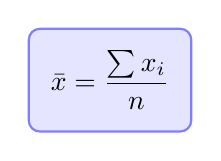
\begin{tikzpicture}
\node[rectangle, fill=blue!10, rounded corners, inner sep=8pt, draw=blue!50, thick] (box) {
$\displaystyle \bar{x} = \frac{\sum x_i}{n}$
};
\end{tikzpicture}

\vspace{0.3cm}

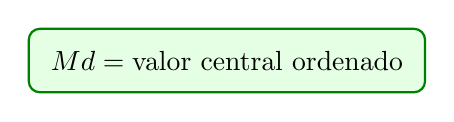
\begin{tikzpicture}
\node[rectangle, fill=green!10, rounded corners, inner sep=8pt, draw=green!50!black, thick] (box) {
$\displaystyle Md = \text{valor central ordenado}$
};
\end{tikzpicture}

\vspace{0.3cm}

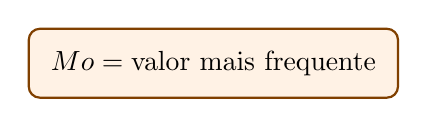
\begin{tikzpicture}
\node[rectangle, fill=orange!10, rounded corners, inner sep=8pt, draw=orange!50!black, thick] (box) {
$\displaystyle Mo = \text{valor mais frequente}$
};
\end{tikzpicture}
\end{center}

\vspace{0.5cm}
\textcolor{blue}{\textbf{Legenda:}} 
\begin{itemize}
\item \textcolor{blue}{Respostas numéricas:} \respostaNum{exemplo}
\item \textcolor{blue}{Respostas textuais:} \textcolor{blue}{exemplo}
\end{itemize}

\end{multicols}

\end{document}
